\newcommand{\be}{\mathbf{e}}
\newcommand{\T}{\mathscr{T}}
\newcommand{\V}{\mathbb{V}}
\newcommand{\mm}{\mathcal{M}}
\newcommand{\nn}{\mathcal{N}}
\newcommand{\parent}[1]{\left( #1 \right)}
\newcommand{\dx}{\mathrm{d}x}
\newcommand{\dr}{\mathrm{d}r}
\newcommand{\dd}{\mathrm{d}}
\newcommand{\Id}{\mathrm{Id}}
\newcommand{\suave}[1]{\mathscr{C}^{\infty}\parent{#1}}

\newcommand{\bee}{\widetilde{\be}}
\newcommand{\Rmm}[4]{\Rm\parent{#1,#2}#3, #4}
\newcommand{\segf}{\mathbf{\mathrm{\RNum{2}}}}
\newcommand{\RNum}[1]{\textbf{\uppercase\expandafter{\romannumeral #1\relax}}}
\newcommand{\conj}[2]{\{#1 \ \vert \ #2 \}}
\newcommand{\tioC}[2]{\widetilde{#1}^{#2}}
\newcommand{\tioB}[2]{\widetilde{#1}_{#2}}
\newcommand{\Munderbrace}[2]{\begingroup \color{violet} \underbrace{\color{black} #1 }_{\color{violet} #2 } \endgroup}
\newcommand{\Bunderbrace}[2]{\begingroup \color{gal} \underbrace{\color{black} #1 }_{\color{gal} #2 } \endgroup}
\newcommand{\Moverbrace}[2]{\begingroup \color{violet} \overbrace{\color{black} #1 }^{\color{violet} #2 } \endgroup}
\renewcommand{\l}{\ell}

\newcommand{\tr}{\operatorname{tr}}
\newcommand{\Ric}{\mathrm{Ric}}
\newcommand{\Rm}{\mathrm{Rm}}
\newcommand{\Lip}{\mathrm{Lip}}
\newcommand{\dist}{\mathrm{dist}}
\newcommand{\Scal}{\mathrm{Scal}}
\newcommand{\cn}{\nabla}
\newcommand{\KN}{\mathbin{\bigcirc\mspace{-15mu}\wedge\mspace{4mu}}}

\newcommand{\emvioleta}[1]{\textbf{\textcolor{violet}{#1}}}

\documentclass[a4paper, 12pt, twoside]{article}
\usepackage[utf8]{inputenc}
\usepackage[T1]{fontenc}
\usepackage[portuguese]{babel}
\usepackage[dvipsnames]{xcolor}
\usepackage{amsmath, amsfonts}
\usepackage{amsthm}
\usepackage{etoolbox}
\usepackage{lmodern}
\usepackage{lastpage}
\usepackage{totcount}
\everymath{\displaystyle}
%\usepackage[sc]{mathpazo}
%\linespread{1.05} 
\usepackage{mathrsfs}
\usepackage{faktor}


\definecolor{navybluegalaxy}{RGB}{0, 36, 93}
\newcommand{\bigslant}[2]{{\raisebox{.2em}{$#1$}\left/\raisebox{-.2em}{$#2$}\right.}}

\newcommand{\mycitep}[1]{{\color{teal}\textbf{\cite{#1}}}}
\definecolor{gal}{RGB}{0, 7, 111}






\makeatletter
\patchcmd{\f@nch@head}{\rlap}{\color{BlueViolet}\rlap}{}{}
%\patchcmd{\headrule}{\hrule}{\color{TealBlue}\hrule}{}{}
\patchcmd{\f@nch@foot}{\rlap}{\color{BlueViolet}\rlap}{}{}
\patchcmd{\footrule}{\hrule}{\color{green}\hrule}{}{}
\makeatother

\newtheorem{exerc}{Questão}
\usepackage{float,framed}
\setlength{\intextsep}{2pt}
\setlength{\textfloatsep}{2pt}
\newfloat{Box}{H}{0ob}
\newenvironment{Mybox}{\begin{Box}\begin{framed}\begin{exerc}}{\end{exerc}\end{framed}\end{Box}}



%\usepackage[shortlabels]{enumitem}

\usepackage[a4paper,bottom=0.9in,top=0.9in,left=0.3in,right=0.3in]{geometry}

\usepackage{mathtools}
\usepackage{fancyhdr}
\usepackage{lipsum}
\usepackage{enumerate}
\usepackage{enumitem}

\usepackage{lastpage}
\usepackage{graphicx}
\everymath{\displaystyle}
\newcommand{\p}{\partial}
\pagestyle{fancy}
%\renewcommand{\footrulewidth}{0.4pt}
\fancyhf{}
%\rhead{\color{BlueViolet}\textbf{2022/1}}
%\chead{\textbf{\thepage}}
\lhead{\color{BlueViolet}\textbf{\textit{Um passeio histórico}}}
\lfoot{\textbf{MATHEUS A. R. M. HORÁCIO}}
%\rfoot{\textbf{MATRÍCULA: 17/0110923 }}
\rfoot{\textbf{Página \thepage \ de \pageref*{LastPage}}}
  \renewcommand\headrule{%

 \color{BlueViolet}\noindent\makebox[\linewidth]{\rule{\paperwidth}{1pt}}
}
  \renewcommand\footrule{%

 \color{BlueViolet}\noindent\makebox[\linewidth]{\rule{\paperwidth}{1pt}}
}




\newcommand{\om}{\mathbb{M}}

\newcommand{\jps}[1]{\textcolor{blue}{#1}}
%\newcommand{\red}[1]{\textcolor{red}{#1}}
\newcommand{\pur}[1]{\textcolor{purple}{#1}}
\newcommand{\maggg}[1]{\textcolor{magenta}{#1}}

%\usepackage{color}
%\definecolor{SAEblue}{rgb}{0, .62, .91}
%\renewcommand\theequation{\red{{\arabic{equation}}}}


\makeatletter
\let\mytagform@=\tagform@
\def\tagform@#1{\maketag@@@{\bfseries\jps{(\ignorespaces#1\unskip\@@italiccorr)}}\hspace{3mm}}
\renewcommand{\eqref}[1]{\textup{\mytagform@{\ref{#1}}}}
\makeatother


%\chead{\textbf{\thepage}}
\theoremstyle{definition}
\newtheorem{def*}{Definição}
\newtheorem{quest}{Questão}
\newtheorem{quest2}{Questão}
\newcommand{\ve}{\varepsilon}
\newcommand{\lnr}{\left\|}
\newcommand{\ssum}{\displaystyle\sum}
\newcommand{\rnr}{\right\|}
%\newcommand{\R}{\mathbb{R}}
\newcommand{\C}{\mathbb{C}}
\DeclareMathOperator{\hol}{Hol}
\newtheorem*{obs*}{Notação}
%\newtheorem*{oobs}{Observação}
\newtheorem{sublema}{Sub-lema}
\renewcommand{\qedsymbol}{\rule{0.7em}{0.7em}}
\newenvironment{demm}{\smallskip \noindent{\bf \underline{Demonstração:}}}
{\begin{flushright} $\qedsymbol$\end{flushright}\smallskip}


\allowdisplaybreaks

\usepackage{tikz}

\newcommand\PlaceText[3]{%
\begin{tikzpicture}[remember picture,overlay]
\node[outer sep=0pt,inner sep=0pt,anchor=south west] 
  at ([xshift=#1,yshift=-#2]current page.north west) {#3};
\end{tikzpicture}%
}


\newtheoremstyle{theoremDEF}% name of the style to be used
  {\topsep}% measure of space to leave above the theorem. E.g.: 3pt
  {\topsep}% measure of space to leave below the theorem. E.g.: 3pt
  {}% name of font to use in the body of the theorem
  {1pt}% measure of space to indent
  {\bfseries\color{cyan}}% name of head font
  {}% punctuation between head and body
  { }% space after theorem head; " " = normal interword space
  {\underline{\thmname{#1} (\thmnumber{D.#2})\textbf{\thmnote{ (#3)}.}}}

\theoremstyle{theoremDEF}
\newtheorem{deff}{Definição}

\newtheoremstyle{theoremEX}% name of the style to be used
  {\topsep}% measure of space to leave above the theorem. E.g.: 3pt
  {\topsep}% measure of space to leave below the theorem. E.g.: 3pt
  {}% name of font to use in the body of the theorem
  {1pt}% measure of space to indent
  {\bfseries\color{BlueViolet}}% name of head font
  {}% punctuation between head and body
  { }% space after theorem head; " " = normal interword space
  {\underline{\thmname{#1} (\thmnumber{E.#2})\textbf{\thmnote{ (#3)}.}}}

\theoremstyle{theoremEX}
\newtheorem{exem}{Exemplo}

\newtheoremstyle{theoremOOBS}% name of the style to be used
  {\topsep}% measure of space to leave above the theorem. E.g.: 3pt
  {\topsep}% measure of space to leave below the theorem. E.g.: 3pt
  {}% name of font to use in the body of the theorem
  {1pt}% measure of space to indent
  {\bfseries\color{violet}}% name of head font
  {}% punctuation between head and body
  { }% space after theorem head; " " = normal interword space
  {\underline{\thmname{#1} (\thmnumber{O.#2})\textbf{\thmnote{ (#3)}.}}}

\theoremstyle{theoremOOBS}
\newtheorem{oobs}{Observação}


\newtheoremstyle{theoremNOT}% name of the style to be used
  {\topsep}% measure of space to leave above the theorem. E.g.: 3pt
  {\topsep}% measure of space to leave below the theorem. E.g.: 3pt
  {}% name of font to use in the body of the theorem
  {1pt}% measure of space to indent
  {\bfseries\color{cyan}}% name of head font
  {}% punctuation between head and body
  { }% space after theorem head; " " = normal interword space
  {\underline{\thmname{#1} (\thmnumber{N.#2})\textbf{\thmnote{ (#3)}.}}}

\theoremstyle{theoremNOT}
\newtheorem{nott}{Notação}


\newtheoremstyle{theoremLEM}% name of the style to be used
  {\topsep}% measure of space to leave above the theorem. E.g.: 3pt
  {\topsep}% measure of space to leave below the theorem. E.g.: 3pt
  {}% name of font to use in the body of the theorem
  {1pt}% measure of space to indent
  {\bfseries\color{navybluegalaxy}}% name of head font
  {}% punctuation between head and body
  { }% space after theorem head; " " = normal interword space
  {\underline{\thmname{#1} (\thmnumber{L.#2})\textbf{\thmnote{ (#3)}.}}}

\theoremstyle{theoremLEM}
\newtheorem{lema}{Lema}

\newtheoremstyle{theoremTEO}% name of the style to be used
  {\topsep}% measure of space to leave above the theorem. E.g.: 3pt
  {\topsep}% measure of space to leave below the theorem. E.g.: 3pt
  {\itshape}% name of font to use in the body of the theorem
  {5pt}% measure of space to indent
  {\bfseries\color{gal}}% name of head font
  {}% punctuation between head and body
  { }% space after theorem head; " " = normal interword space
  {\underline{\thmname{#1} (\thmnumber{T.#2})\textbf{\thmnote{ (#3)}.}}}
  


\theoremstyle{theoremTEO}
\newtheorem{teorema}{Teorema}

\newtheoremstyle{theorempergunta}% name of the style to be used
  {\topsep}% measure of space to leave above the theorem. E.g.: 3pt
  {\topsep}% measure of space to leave below the theorem. E.g.: 3pt
  {}% name of font to use in the body of the theorem
  {1pt}% measure of space to indent
  {\bfseries\color{gal}}% name of head font
  {}% punctuation between head and body
  { }% space after theorem head; " " = normal interword space
  {\underline{\thmname{#1} (\thmnumber{P.#2})\textbf{\thmnote{ (#3)}.}}}


\theoremstyle{theorempergunta}
\newtheorem{pergunta}{Pergunta}




\usepackage{csquotes}
\usepackage{lettrine}
\newcommand{\quotes}[1]{``#1''}
\newcommand{\bl}[1]{\textnormal{\textcolor{black}{#1}}}
\newcommand{\colch}[1]{\left\{ #1 \right\}}



\makeatletter
\let\NAT@parse\undefined
\makeatother


\usepackage{hyperref}
\hypersetup{
	pagebackref=true,
    colorlinks=true, %set true if you want colored links
    linktoc=all,     %set to all if you want both sections and subsections linked
    linkcolor=black,
    citecolor = teal  %choose some color if you want links to stand out
}

\usepackage{cleveref}


\crefname{deff}{}{definitions}
\crefname{exem}{}{exemplos}
\crefname{col}{}{corolários}
\crefname{equation}{}{equações}
\creflabelformat{equation}{#2{\bf{\color{blue}(#1)}}#3}
\crefname{teorema}{}{teoremas}
\crefname{oobs}{observação}{observações}
\creflabelformat{oobs}{#2\bf{\color{violet}(O.#1)}#3}
\crefname{lema}{}{lemas}
\creflabelformat{lema}{#2\bf{\color{gal}(L.#1)}#3}
\crefname{proposicao}{}{proposições}
\creflabelformat{deff}{#2\bf{\color{cyan}(D.#1)}#3}
\creflabelformat{exem}{#2\bf{\color{BlueViolet}(E.#1)}#3}
\creflabelformat{col}{#2\bf{\color{Aquamarine}(C.#1)}#3}
\creflabelformat{proposicao}{#2{\bf\color{Sepia}(P.#1)}#3}
%\renewcommand{\theenumi}{\Alph{enumi}}

\newcommand{\Hess}{\text{Hess}}
\newcommand{\grad}{\text{grad}}
\newcommand{\bb}{\mathcal{B}}
\newcommand{\conjunto}[2]{\{#1 \ \vert \ #2 \}}

\newtheoremstyle{theoremconjec}% name of the style to be used
  {\topsep}% measure of space to leave above the theorem. E.g.: 3pt
  {\topsep}% measure of space to leave below the theorem. E.g.: 3pt
  {}% name of font to use in the body of the theorem
  {1pt}% measure of space to indent
  {\bfseries\color{gal}}% name of head font
  {}% punctuation between head and body
  { }% space after theorem head; " " = normal interword space
  {\underline{\thmname{#1.} \thmnumber{}\textbf{\thmnote{}}}}

\theoremstyle{theoremconjec}
\newtheorem{conjec}{A conjectura da geometrização de Thurston}

\crefname{pergunta}{}{perguntas}
\creflabelformat{pergunta}{#2\bf{\color{gal}(P.#1)}#3}




\setlength{\parindent}{3em}
\setlength{\parskip}{.2em}
\begin{document}

\PlaceText{69mm}{38mm}{ \color{gal}\noindent\makebox[\linewidth]{\rule{2\paperwidth}{1pt}}}

\PlaceText{69mm}{14.3mm}{ \color{white}\noindent\makebox[\linewidth]{\rule{2\paperwidth}{12pt}}}

\PlaceText{69mm}{15mm}{ \color{gal}\noindent\makebox[\linewidth]{\rule{2\paperwidth}{1pt}}}

\PlaceText{69mm}{19mm}{ \color{white}\noindent\makebox[\linewidth]{\rule{2\paperwidth}{3pt}}}

\PlaceText{67mm}{31mm}{\Huge \textcolor{gal}{\textit{Um passeio histórico}}}

%\vspace{1cm}

\lettrine[nindent=2em,lines=1]{N} as palavras de Carl Sagan, o Cosmos é tudo o que existe, existiu ou existirá. A teoria da relatividade geral de Einstein modela o Cosmos como uma variedade pseudo-Riemanniana de dimensão $4$ (com $3$ dimensões espaciais e $1$ temporal), cujos efeitos gravitacionais podem ser explicados pela curvatura de tal variedade, que é comumente chamada de \textit{espaço-tempo}. Explicitamente, em tal modelo a gravidade não pode ser considerada como uma força no sentido convencional: na verdade, ela é uma propriedade intrínseca do espaço-tempo e \quotes{nasce} como resultado de sua curvatura local, que por sua vez reage à distribuição de massa-energia, momento e stress de uma região espacial via a seguinte equação:
\begin{equation}\label{efe}
\Ric - \frac{1}{2} \cdot \Scal \cdot g + \Lambda g = \frac{8 \pi G}{c^4} T
\end{equation}
onde $T$ denota o tensor de energia-momento do espaço-tempo e as constantes $\Lambda, G$ e $c$ denotam, respectivamente, a \emph{constante cosmológica} do modelo, a constante Newtoniana de gravitação, e a velocidade da luz no vácuo. Na verdade, a convenção de denotar a métrica Riemanniana por $g$ foi originada por Einstein e Grossman por volta de 1910-13, que perceberam que as componentes $\{g_{\mu \nu} \}_{1 \leq \mu, \nu \leq 4}$ que determinam a geometria do espaço-tempo pareciam depender da quantidade de máteria em gravitação da região estudada. E como visto em \mycitep{foster}, há um sentido preciso em que as quantidades $\{g_{\mu \nu} \}_{1 \leq \mu, \nu \leq 4}$ podem ser vistas como potenciais gravitacionais. Geralmente, a equação \cref{efe} é apresentada em coordenadas locais, na forma
\[
\Ric_{\mu \nu} - \frac{1}{2} \cdot \Scal \cdot g_{\mu \nu} + \Lambda g_{\mu \nu} = \frac{8 \pi G}{c^4} T_{\mu \nu}
\]
que ao todo constituem um sistema de $10$ equações diferenciais parciais (onde o $10$ vem do fato de que os tensores envolvidos têm $10$ componentes independentes, conforme visto em \mycitep{ivoQ}). \par 
Sendo assim, podemos muito bem fazer a seguinte:

\begin{pergunta}\label{FibUniverso}
\textit{Dada uma fibração (a pergunta de qual fibração exatamente devemos considerar é mais sutil e por simplicidade pode ser negligenciada - mas vale a pena mencionarmos que a existência da radiação cósmica de fundo em microondas e o príncipo copérnico de certa forma implicam na existência de uma fibração canônica) do Cosmos por \quotes{fatias temporais} tri-dimensionais (todas isométricas entre si, sendo uma tal fibra denominada de Universo), quais são todas as topologias e geometrias possíveis de tais fatias?}
\end{pergunta} 
 \par Em outras palavras, se $\mm^3$ é uma variedade topológica tri-dimensional, existem um conjunto finito $\mathcal{F}$  de classes de equivalência de variedades (onde a relação de equivalência é determinada ao declararmos que duas variedades são equivalentes quando são homeomorfas), uma métrica Riemanniana $g \in \Gamma(\text{Sym}_2^{+} \mm^3)$ e um conjunto finito de classes de equivalência de métricas Riemannianas $\mathcal{G}$ (onde nesse caso a relação de equivalência é determinada ao declararmos que duas métricas são equivalentes quando são isométricas) tal que $\left[\mm^3 \right] \in \mathcal{F}$, $[g] \in \mathcal{G}$? Veremos que a resposta é negativa, mas conseguiremos chegar razoavelmente perto. Se não assumirmos que $\mm^3$ é compacta, o problema é demasiadamente difícil: por exemplo, McMillan provou em \mycitep{McMillan} que existe um conjunto não-enumerável $\mathfrak{F}$ de subconjuntos de $\mathbb{R}^3$ abertos e contratéis tais que $[X] \neq [Y]$ sejam quais forem $X \neq Y \in \mathfrak{F}$. Por simplicidade, assumiremos então que $\mm^3$ é compacta e sem bordo.  \par
 Uma primeira impressão ingênua é de que perguntas especulativas desse tipo, que nascem puramente da abstração matemática, não possam possivelmente ter consequências físicas reais e observáveis no nosso próprio universo. Porém, o próprio estudo da geometria diferencial clássica de superfícies indica fortemente que esse \emph{não} é o caso. Por exemplo, usamos inconscientemente o teorema Egregium de Gauss toda vez que dobramos um livro a fim de conseguir lê-lo segurando com uma mão só, ou quando dobramos um pedaço de pizza para conseguirmos comê-lo sem o mesmo cair. \emph{Curvatura cria força} é um dos princípios físicos impostos pelo teorema Egregium de Gauss que tanto engenheiros ao redor do mundo como a própria natureza usam em suas construções. Veja, por exemplo, o formato de usinas nucleares ou de fios de capim.  \par
É claro que o modelo relatívistico do Cosmos não é um retrato completamente fiel da realidade. O Cosmos pode ser algo muito mais complexo do que uma variedade pseudo-Riemanniana, e no futuro distante pode muito bem acontecer que algum matemático ou físico descubra espaços mais gerais que tenham as variedades como as conhecemos hoje como casos particulares e o modelem com mais precisão do que o modelo relativístico. Porém, isso não constitui nenhuma grande perda, afinal o próprio modelo da Terra como sendo a esfera redonda $\mathbb{S}^2$ também não é completamente preciso: a Terra é achatada nos polos, e a existência de milhares de arcos naturais mostra também que o seu gênero é no mínimo na ordem de $10^3$.\par
  Observe ainda que pela teoria da relatividade, o conceito de \quotes{fatias temporais} a priori não está bem definido: afinal, o próprio conceito de simultaneidade não é absoluto e depende do referencial de cada observador. Por exemplo, poderíamos perguntar: a idade do universo (conhecidamente $\approx 14 \times 10^9$ anos) é comumente medida com respeito a qual observador? Felizmente, o uso de \emph{coordenadas comóveis} toma conta desse problema e torna tais conceitos bem postos. Em particular, a idade do universo é medida com respeito a um observador com zero velocidade comóvel - qualquer tal observador percebe todo o universo como isotrópico (na verdade, somente tais observadores o percebem assim) -, ou seja, $ \approx 14 \times 10^9$ anos é o tempo passado desde o Big Bang de acordo com o relógio de um observador comóvel. \par 
Antes de nos aprofundarmos no problema de classificação em dimensão $3$, podemos analisar o que acontece nos casos de dimensão menor - ou seja, quais são todas as topologias e geometrias possíveis de mundos (variedades uni/bi-dimensionais compactas e sem bordo) de dimensão $\leq 2$? Tal pergunta é primordial e foi, de certa forma, contemplada pelos gregos há mais de dois mil e duzentos anos - daí que vem a origem da palavra \quotes{geometria}, que significa \quotes{medir} a Terra. É claro que hoje é possível embarcar numa nave espacial e observar diretamente o formato redondo da Terra. Os antigos gregos, porém, não tinham essa opção (e obviamente, também jamais teremos tal opção para observar a topologia do espaço-tempo, de forma que métodos intrínsecos se tornam absolutamente necessários). Tales de Mileto acreditava que a Terra era um disco plano flutuando num oceano gigante, enquanto que Anaximandro, discípulo de Tales, pensava que a Terra tinha a forma de um cilindro, onde os continentes estavam localizados numa de suas faces circulares. Porém, foi Aristarco de Samos, um astrônomo e matemático grego que viveu entre $310$ a.C. e $230$ a.C, na sua fantástica obra \emph{Sobre os tamanhos e distâncias entre o Sol e a Lua}, que pavimentou o caminho para que Eratóstenes, outro grande cientista grego, pudesse atacar tal problema com grande êxito, ao, entre outras descobertas, observar que os raios solares eram paralelos. \par 
Eratóstenes foi diretor da biblioteca de Alexandria, um dos maiores centros de conhecimento da Antiguidade. Por meio de um dos manuscritos da biblioteca, ele tomou conhecimento de um fenômeno notável que acontecia no Solstício de Verão de 21 de junho: pela manhã, em Siena (atual Assuão), as sombras das colunas dos templos (ou de uma vara verticalmente fixada no chão, por exemplo) iam diminuindo cada vez mais à medida que o meio-dia se aproximava. Precisamente na chegada do meio-dia, tais colunas não lançavam sombra alguma - analogamente, um poço profundo de água, que nos outros dias do ano era inteiramente coberto pela sombra, ficava completamente iluminado pelo Sol, que brilhava nitidamente na água do poço (esse instante, em que o sol está exatamente no \quotes{topo} do céu, se chama zênite solar). \par 
Tal observação, que a princípio poderia parecer insignificante, se provou muito frutífera: Eratóstenes teve a sagacidade de se perguntar se o mesmo fenômeno acontecia simultaneamente também em Alexandria. Ele descobriu que não - no mesmo dia, em Alexandria, colunas de templos lançavam suas longas sombras usuais. Eratóstenes se perguntou como poderia acontecer de, no mesmo instante, uma vara em Siena não lançar sombra alguma enquanto que, 800 quilômetros ao norte, em Alexandria, uma vara lançava uma sombra muito definida. Numa Terra plana a uma distância suficientemente grande do Sol (hipótese essa de fato atestada por Aristarco de Samos), a presença ou ausência de sombras necessariamente deveria ser vista simultaneamente em quaisquer lugares. Consequentemente, a presença substancial de sombras em Alexandria conjuntamente com sua ausência em Siena demonstravam a curvatura da Terra. \par 
Além disso, quanto maior a curvatura, maior a diferença no comprimento das sombras: pois, como já tinha sido observado por Aristarco de Samos, os raios solares são paralelos, e portanto, varas cujos ângulos com o Sol são distintos lançarão sombras de comprimentos diferentes. Era portanto razoável supor a esfericidade da Terra. Munido de tal hipótese e usando trigonometria, Eratóstenes calculou que a diferença observada no comprimento das sombras implicava que a distância entre Alexandria e Siena correspondia a aproximadamente sete graus ao longo da superfície da Terra (ou seja, imaginando-se que as varas em Alexandria e Siena fossem estendidas até o centro da Terra, as mesmas se intersectariam num ângulo de aproximadamente sete graus). Uma vez que sete graus corresponde a aproximadamente um quinquagésimo de uma circunferência inteira, Eratóstenes estimou a circunferência da Terra como sendo cinquenta vezes a distância entre Alexandria e Siena, que na época era estimada como cinco mil estádios - e portanto a circunferência da Terra era aproximadamente duzentos e cinquenta mil estádios. A medida precisa de um estádio é desconhecida até hoje (variando desde 157 a 209 metros), mas de qualquer forma, a precisão do cálculo de Eratóstenes para a sua época é incrível, e atesta o poder da engenhosidade humana. \par 
Erroneamente, Eratóstenes ficou conhecido como a primeira pessoa a provar a esfericidade da Terra: na verdade, o sucesso de seu experimento precisou fortemente da suposição a priori de tal esfericidade, e a única conclusão definitiva possível além do diâmetro da Terra foi poder descartar uma possível Terra plana. Outros formatos (i.e. \emph{topologias}) ainda eram possíveis: poderia acontecer que o  mundo se estendesse indefinidamente, ou até mesmo que tivesse um fim (i.e. um \emph{bordo} topológico). Tais hipóteses foram descartadas pela primeira circum-navegação do globo, feita por Fernão Magalhes no século $16$, mas ainda assim outros formatos não-esféricos ainda não podiam ser descartados, uma vez que nem todas as regiões do mundo, incluindo os polos, tinham sido mapeadas. Os mapas de Battista Agnese eram razoavelmente consistentes com uma Terra toroidal, por exemplo (para detalhes, consulte \mycitep{Donal}), e sabemos hoje que um planeta toroidal não é fisicamente impossível, mesmo que nenhum tenha sido descoberto. \par 
Feita essa digressão, voltemos agora ao problema sob uma perspectiva inteiramente matemática: quais são todas as topologias possíveis de uma superfície Riemanniana fechada, e qual a relação dessas com a geometria? Para abordar tais problemas, será útil explorarmos os seguintes conceitos antes: 
\begin{itemize}
\item \emph{a soma conexa} de duas variedades fechadas: dadas duas variedades fechadas $\mm$ e $\nn$, existe uma maneira de construir uma nova variedade chamada da \emph{soma conexa} de $\mm$ e $\nn$, que denotaremos por $\mm \sharp \nn$. Escolhemos duas bolas $V_1, V_2$, em $\mm$ e $\nn$ respectivamente, pequenas o suficiente de forma a serem homeomorfas a bolas. Em seguida removemos o interior dessas duas bolas, resultando em dois bordos $\partial V_1$ e $\partial V_2$ homeomorfos a $\mathbb{S}^n$. Ao colar tais conjuntos e identificar tais bordos via um difeomorfismo $\psi: V_1 \to V_2$ que reverte orientação, obtemos uma nova variedade conexa. Formalmente, 
\[
\mm \sharp \nn = \frac{(\mm \setminus \text{int}(V_1)) \sqcup (\nn \setminus \text{int}(V_2))}{p \in \partial V_1 \sim \psi(p) \in \partial V_2}
\] Pode-se provar que tal operação está bem definida, é compatível com a orientação de cada fator, é associativa e comutativa, em geral não possui inverso e tem a esfera como elemento neutro. Algumas visualizações úteis são as seguintes
\begin{figure}[H]
\centering
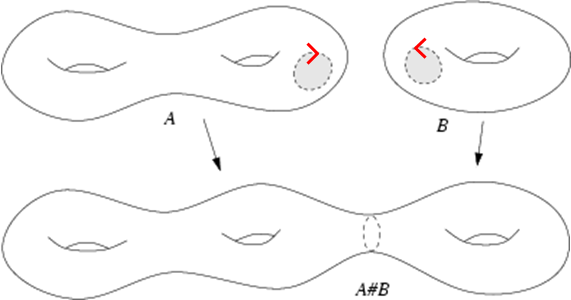
\includegraphics[scale=.5]{somaconexa.png}
\caption{a soma conexa de um toro com um bi-toro}
\end{figure}
\begin{figure}[H]
\centering
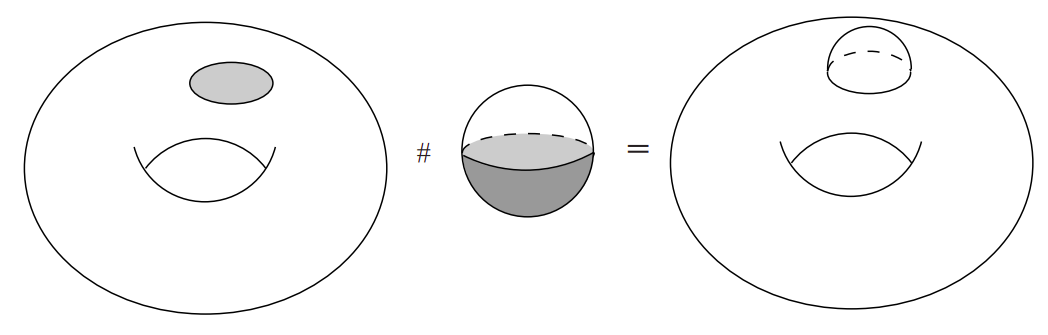
\includegraphics[scale=.33]{SomaEsfera.png}
\caption{a soma conexa de um toro com uma esfera}
\end{figure}
\item \emph{a representação poligonal} de uma superfície compacta: uma representação polígonal de uma superfície é um polígono onde cada lado possui um rótulo e direção (comumente representada como uma seta). Quando dois lados têm o mesmo rótulo, isso indica que os mesmos devem ser \quotes{colados} usando um homeomorfismo compatível com a direção das setas correspondentes. Por exemplo, 
\begin{figure}[H]
\centering
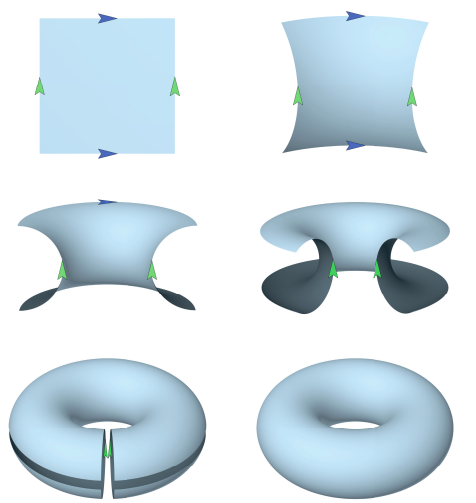
\includegraphics[scale=.55]{torojeff.png}
\caption{a representação poligonal do toro $\mathbb{T}^2 = \mathbb{S}^1 \times \mathbb{S}^1$}
\end{figure}

\begin{figure}[H]
\centering
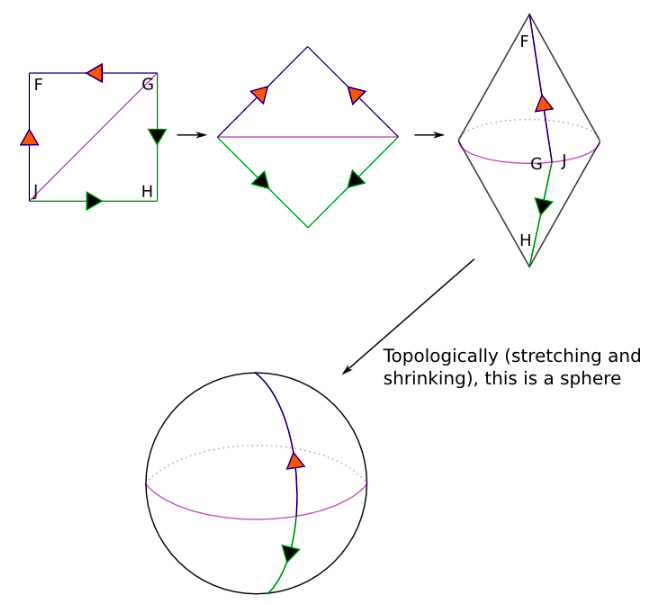
\includegraphics[scale=.5]{RepDaEsfera.png}
\caption{a representação poligonal da esfera $\mathbb{S}^2$}
\end{figure}

\begin{figure}[H]
\centering
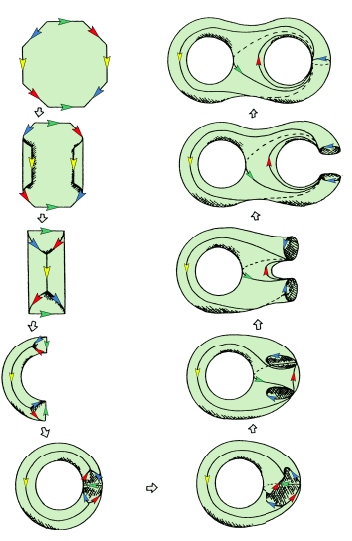
\includegraphics[scale=.6]{bitoro.png}
\caption{a representação poligonal do bitoro $\mathbb{T}^2 \sharp \mathbb{T}^2$}
\end{figure}
\vspace{1cm}
\begin{figure}[H]
\centering
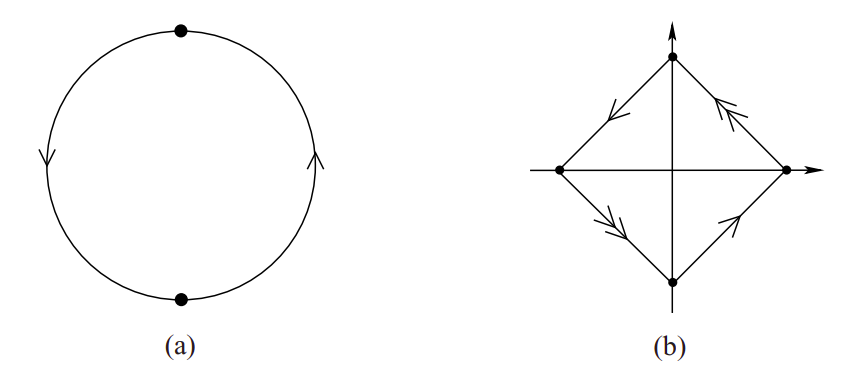
\includegraphics[scale=.6]{projetivo.png}
\caption{representações poligonais do plano projetivo $\mathbb{R}\mathbb{P}^2$}
\end{figure}
\end{itemize}
É possível mostrar que toda superfície compacta admite uma representação polígonal.  Em geral, temos o seguinte:
\begin{teorema}\label{CLASS}
\textit{Toda variedade bi-dimensional $\mm^2$ conexa e fechada é homeomorfa a exatamente um dos seguintes espaços:
\begin{itemize}
\item a esfera $\mathbb{S}^2$
\item a soma conexa finita de uma ou mais cópias do toro $\mathbb{T}^2 = \mathbb{S}^1 \times \mathbb{S}^1$
\item a soma conexa finita de uma ou mais cópias do plano projetivo $\mathbb{R}\mathbb{P}^2$
\end{itemize}
}
\end{teorema}

É difícil superestimar a importância do teorema \cref{CLASS}. Nas palavras de V.I. Arnold (veja \mycitep{Arnold}), um dos maiores matemáticos do século passado,
\blockquote{The theorem of classification of surfaces is a top-class mathematical achievement, comparable with the discovery of America or X-rays. This is a genuine discovery of mathematical natural science and it is even difficult to say whether the fact itself is more attributable to physics or to mathematics. In its significance for both the applications and the development of correct Weltanschauung it by far surpasses such \quotes{achievements} of mathematics as the proof of Fermat's last theorem or the proof of the fact that any sufficiently large whole number can be represented as a sum of three prime numbers.}

Em dimensão $2$, a geometria e topologia determinam uma à outra pelas seguintes consequências diretas do teorema da uniformização e do teorema de Gauss-Bonnet, enunciados a seguir:
\begin{teorema}
Toda superfície fechada $\mm^2$ admite uma métrica Riemanniana de curvatura seccional constante.
\end{teorema}
\begin{teorema} A curvatura total de uma variedade bi-dimensional $\mm^2$ satisfaz:
\[
\int_{\mm^2} K \ \mathrm{d} A = 2 \pi \cdot \chi(\mm^2)
\]
\end{teorema}
Consequentemente, a característica de Euler e a orientabilidade são invariantes topológicos que determinam completamente a topologia de uma superfície fechada. As de gênero $0$ admitem geometria esférica, e as de gênero $1$ a plana (o toro, por exemplo, admite uma métrica de curvatura zero obtida ao \quotes{descer} a métrica do recobrimento $\mathbb{R}^2$ ao toro $\mathbb{T}^2$). Todas as outras, de gênero $g >1$, são modeladas pela geometria hiperbólica, que é nesse sentido abundante - e infelizmente impossível de visualizar fielmente, devido ao teorema de Hilbert. A construção de tais métricas hiperbólicas nasce de um polígono com $4g$ lados com identificações apropriadas, onde todos os vértices são identificados com um único ponto. É necessário portanto que a soma dos ângulos internos de tal polígono seja igual a $2 \pi$. Note que os ângulos da geometria Euclidiana são \quotes{gordos} demais para gerar qualquer métrica hiperbólica: de fato, 
\[
(4g - 2) \pi > 2 \pi, \ \forall g \geq 2
\] Por outro lado, no disco de Poincaré, a soma dos ângulos internos de um polígono hiperbólico é dada por
$$(4g - 2) \pi - A$$
onde $A$ denota a área do polígono. Portanto existem polígonos hiperbólicos de ângulos internos $\frac{2 \pi}{4g}$, de forma que toda superfície fechada de gênero $g > 1$ admite uma métrica hiperbólica.
\begin{figure}[H]
\centering
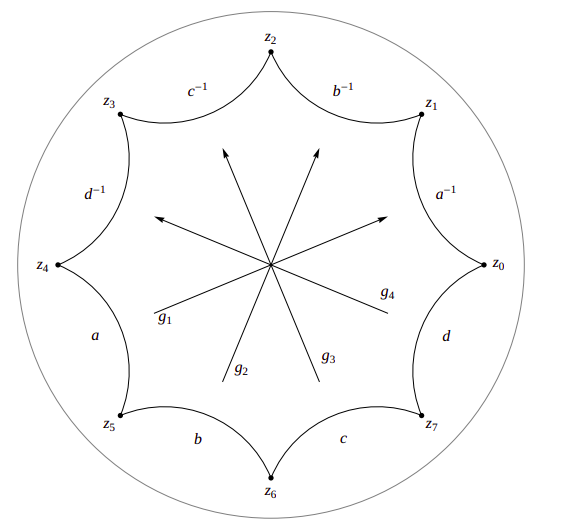
\includegraphics[scale=.5]{HypOct.png}
\caption{octágono hiperbólico com identificações rotuladas que geram o bi-toro com geometria hiperbólica}
\end{figure}
\par 
Em dimensão $1$, a situação é consideravelmente mais simples: qualquer variedade (conexa) de dimensão $1$ sem bordo é difeomorfa ou ao círculo $\mathbb{S}^1$ ou à reta real $\mathbb{R}$. A presença de bordo introduz os casos adicionais $[0, 1]$ e $[0, 1)$. Compacidade e a presença de bordo são portanto invariantes topológicos que juntos determinam completamente variedades de dimensão $1$. Além disso, nenhuma variedade Riemanniana unidimensional possui geometria intrínseca: em virtude da definição do tensor curvatura, em dimensão $1$ a curvatura sempre é identicamente nula, de forma que qualquer variedade Riemanniana uni-dimensional é localmente isométrica a $\mathbb{R}$ (mas é claro - um tensor antissimétrico em dimensão $1$ necessariamente é identicamente nulo!).
 \par 
A situação em dimensão $3$ se torna interessantíssima: antes da incrível teoria da relatividade de Einstein se firmar, era comum pensar que a geometria Euclidiana tri-dimensional modelava com completa fidelidade o Universo. Nas palavras do fantástico físico e matemático Roger Penrose em seu livro \mycitep{PEN1} (outra obra incrível do mesmo autor é \mycitep{PEN2}),
\blockquote{The fact that Euclidean geometry seems so accurately to reflect the structure of the \quotes{space} of our world has fooled us (or our ancestors!) into thinking that this geometry is a logical necessity, or into thinking that we have an innate \emph{a priori} intuitive grasp that Euclidean geometry must apply to the world in which we live. (Even the great philosopher Immanuel Kant claimed this.) This real break with Euclidean geometry only came with Einstein's general relativity, which was put forward many years later. Far from Euclidean geometry being a logical necessity, it is an \emph{empirical observational fact} that this geometry applies so accurately -- though not quite exactly -- to the structure of our physical space! Euclidean geometry was indeed, all along, a (SUPERB) \emph{physical theory}. This was in addition to its being an elegant and logical piece of pure mathematics.}
Uma das inúmeras histórias apócrifas sobre Gauss também o retrata medindo os ângulos de um grande triângulo formado pelos picos montanhosos de Hohenhagen, Inselberg e Brocken, num esforço de obter evidências de que a geometria do espaço é não-Euclidiana. Porém, embora Gauss de fato tenha se envolvido no mapeamento do Reino de Hanover entre $1818$ e $1832$ (tendo trabalhado com alguns \quotes{triângulos testes} formados por picos de montanhas), um desvio da geometria Euclidiana grande o suficiente notável na escala da Terra implicaria em distorções enormes numa escala astronômica, que teriam sido notadas muito antes de Gauss. Por outro lado, tal ideia de fato foi muito promissora - em $1829$, Lobachevsky, contemporâneo de Gauss, propôs um teste análogo, feito ao considerar o paralaxe das estrelas Eridan $29$, Rigel e Sirius. Usando um valor de paralaxe de $1.24$ arco-segundos para Sirius, ele concluiu que a soma dos ângulos internos de um triângulo formado pelo sol, pela Terra e por Sirius desviava do valor Euclidiano de $\pi$ radianos por no máximo $0.00000372$ arco-segundos. Apesar disso sugerir fortemente que o espaço pudesse ser Euclidiano, Lobachevsky se absteve de qualquer conclusão definitiva, percebendo que, embora em princípio houvesse a possibilidade de provar o Universo como não-Euclidiano, nunca se poderia definitivamente prová-lo como Euclidiano (sempre se poderia argumentar que a área do espaço usado em um tal experimento foi pequena demais). \par 
Em \mycitep{RIEMANN}, Bernhard Riemann também propôs a possibilidade do Universo ser modelado pela esfera tri-dimensional $\mathbb{S}^3$, 
\blockquote{
In the extension of space-construction to the infinitely great, we must distinguish between \emph{unboundedness} and \emph{infinite extent}, the former belongs to the extent relations, the latter to the measure-relations. That space is an unbounded three-fold manifoldness, is an assumption which is developed by every conception of the outer world; according to which every instant the region of real perception is completed and the possible positions of a sought object are constructed, and which by these applications is for ever confirming itself. The unboundedness of space possesses in this way a greater empirical certainty than any external experience. But its infinite extent by no means follows from this; on the other hand if we assume independence of bodies from position, and therefore ascribe to space constant curvature, it must necessarily be finite provided this curvature has ever so small a positive value. If we prolong all the geodesics starting in a given-surface element, we should obtain an unbounded surface of constant curvature, \emph{i.e.,} a surface which in a \emph{flat} manifoldness of three dimensions would take the form a sphere, and consequently be finite.
}
Em \mycitep{POINCHYP}, o próprio Poincaré imaginou a perspectiva de habitantes de um Universo hiperbólico $\mathbb{H}^3$:
\blockquote{
Suppose, for example, a world enclosed in a large sphere and subject to the following laws: The temperature is not uniform; it is greatest at the centre, and gradually decreases as we move towards the circumference of the sphere, where it is absolute zero. The law of this temperature is as follows: if $R$ be the radius of the sphere, and $r$ the distance of the point considered from the centre, the absolute temperature will be proportional to $R^2 - r^2$. Further, I shall suppose that in this world all bodies have the same coefficient of dilation so that the linear dilatation of any body is proportional to its absolute temperature. Finally, I shall suppose that a body transported from one point to another of different temperature is instantaneously in thermal equilibrium with its new environment. There is nothing in these hypotheses either contradictory or unimaginable. A moving object will become smaller and smaller as it approaches the circumference of the sphere. Let us observe, in the first place that although from the point of view of our ordinary geometry this world is finite, to its inhabitants it will appear infinite. As they approach the surface of the sphere they become colder, and at the same time smaller and smaller. The steps they take are therefore also smaller and smaller, so that they can never reach the boundary of the sphere. If to us geometry is only the study of laws according to which invariable solids move, to these imaginary beings it will be the study of laws of motion \emph{deformed by the differences of temperature alluded to}.... \par 
Let us make another hypothesis: suppose that light passes through media of different refractive indices, such that the index of refraction is inversely proportional to $R^2 - r^2$. Under these conditions it is clear that the rays of light will no longer be rectilinear, but circular.... If they [the beings in such a world] construct a geometry, it will not be like ours, which is the study of movements of our invariable solids; it will be the study of the changes of position which they will have thus distinguished, and will be \quotes{non-Euclidean displacements,} and \emph{this will be non-Euclidean geometry}. So that beings like ourselves, educated in such a world, will not have the same geometry as ours.
} 
Os trabalhos de Gauss e Riemann deram frutos extraordinários: em $1919$, mais de dois mil anos depois do experimento primoridial de Eratóstenes, astronômos britânicos liderados por Arthur Stanley Eddington testaram a teoria da relatividade de Einstein e observaram empiricamente a natureza não-Euclidiana do Cosmos. Eles mediram o ângulo subtendido por duas estrelas e a própria Terra - uma vez quando o Sol não estava bloqueando o caminho da luz de tais estrelas até a Terra e uma vez quando o caminho da luz de uma das estrelas passava muito próximo do Sol (agora tendo que esperar por um eclipse total do Sol, que foi observado tanto pela ilha de Príncipe quanto em solo brasileiro, em Sobral). A diferença entre as duas medições foi exatamente a que a teoria de Einstein previu - que não acontece devido à luz ser de alguma forma distorcida (na verdade, ela segue caminhos intrinsecamente retos - geodésicas!), mas devido à massa enorme do Sol distorcer a geometria do Cosmos nos seus arredores,  precisamente como Einstein previu. \par 
Tais considerações demonstram um pouco da grandiosidade de um possível resultado análogo ao \cref{CLASS} para dimensão $3$, que potencialmente responderia a seguinte
\begin{pergunta}\label{perg1}
\emph{Quais são todas as $3$-variedades fechadas?}
\end{pergunta}
Na busca da resposta, surge um obstáculo inicial imediato: a característica de Euler é um invariante topológico inútil nesse caso - de fato, uma consequência direta da dualidade de Poincaré é que a característica de Euler de qualquer variedade fechada de dimensão ímpar é sempre zero. Na procura de invariantes topológicos em dimensões mais altas, Poincaré praticamente fundou a topologia como a conhecemos atualmente, numa série de seis artigos publicados em jornais renomados. Inicialmente, ele mostrou que o conhecimento dos números de Betti não determinava a topologia de uma variedade, exibindo uma família infinita de variedades tri-dimensionais fechadas que não são homeomorfas entre si, mas com números de Betti idênticos, iguais aos números de Betti de $\mathbb{S}^3$. Alguns de seus primeiros questionamentos foram os seguintes:
\blockquote{
Seria interessante investigar as seguintes perguntas:
\begin{itemize}
\item Dado um grupo $G$ definido por seus geradores e relações, o mesmo pode ser o grupo fundamental de uma variedade $n$-dimensional? 
\item Como tal variedade pode ser formada? 
\item Duas variedades com a mesma dimensão e o mesmo grupo fundamental são sempre homeomorfas? 
\end{itemize}
Essas perguntas envolvem estudos difíceis e desenvolvimentos longos, sobre os quais não falarei aqui.
}
Poincaré tentou responder uma versão muito enfraquecida da pergunta \cref{perg1}: ao invés de tentar caracterizar todas as variedades tri-dimensionais fechadas, ele tentou inicialmente caracterizar a variedade tri-dimensional fechada mais simples de todas - a esfera $\mathbb{S}^3$. No seu primeiro esforço inicial nesse sentido, ele exagerou ao afirmar que qualquer variedade tri-dimensional fechada com \quotes{a homologia de $\mathbb{S}^3$} (\emph{id est} possuindo os mesmos grupos de homologia que $\mathbb{S}^3$) era homeomorfa a $\mathbb{S}^3$, tendo inclusive afirmado que tinha uma prova de tal afirmação. \par 
O próprio Poincaré descobriu o primeiro contra-exemplo de sua afirmação, tendo no processo inventado o conceito do grupo fundamental.  Ele descreveu o contra-exemplo como um par de bi-toros sólidos colados de maneira apropriada (um \emph{diagrama de Heegard}). O espaço resultante tinha não só todos os mesmos grupos de homologia que $\mathbb{S}^3$, mas também grupo fundamental não trivial (e portanto não podia ser homeomorfa à $\mathbb{S}^3$). Atualmente, tal variedade é conhecida como o \emph{dodecaedro} de Poincaré: 
\begin{figure}[H]
\centering
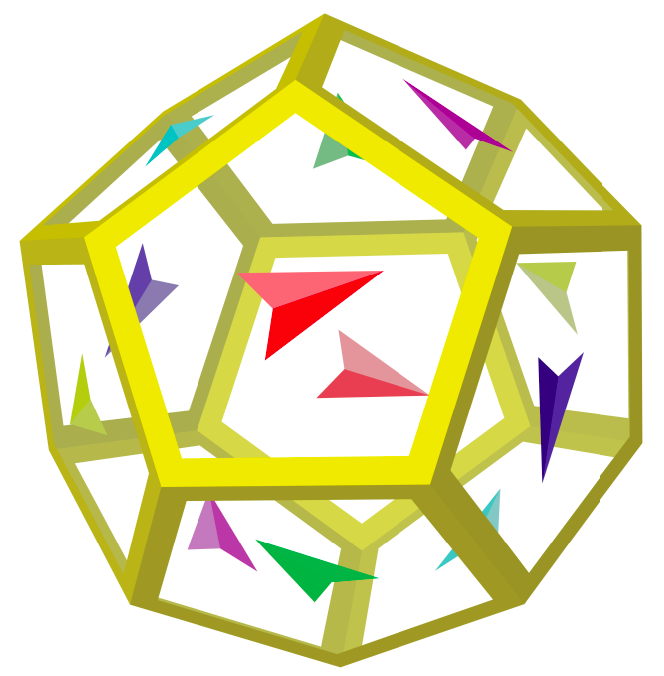
\includegraphics[scale=.4]{dodec.png}
\caption{visualização do dodecaedro de Poincaré - cole faces opostas após um décimo de volta no sentido anti-horário $\left(\text{rotação por $\frac{2 \pi}{10} = \frac{\pi}{5}$ radianos} \right)$}
\end{figure}
A descrição de tal espaço como um dodecaedro com faces opostas identificadas não foi introduzida por Poincaré, mas sim por C.Weber e H.Seifert em \mycitep{dodecaedro}. Recentemente, muita consideração tem sido dada a tal variedade como um possível modelo para a forma/topologia do próprio Universo (veja, por exemplo, \mycitep{ArtDodecaedro}). Com essa identificação das faces, os vinte cantos do dodecaedro Euclidiano se juntam em cinco grupos de quatro, de forma que os seus ângulos internos são \quotes{magros} demais para se encaixarem apropriadamente. Porém, de maneira análoga ao que fizemos para uniformizar a geometria de um bi-toro, podemos considerar um dodecaedro \quotes{esférico} para consertar tal problema, como esboçado na figura abaixo

\begin{figure}[H]
\centering
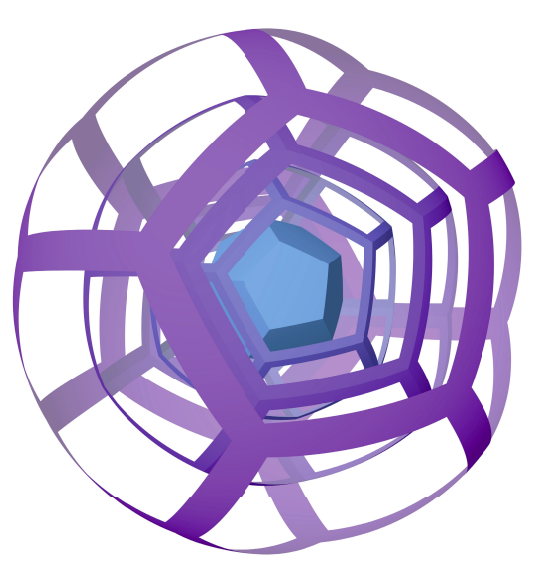
\includegraphics[scale=.3]{edodec.png}
\caption{geometria esférica do dodecaedro de Poincaré: expandimos o dodecaedro imerso em $\mathbb{S}^3$ até os seus cantos terem o tamanho certo para se encaixarme em grupos de quatro}
\end{figure}

\begin{figure}[H]
\centering
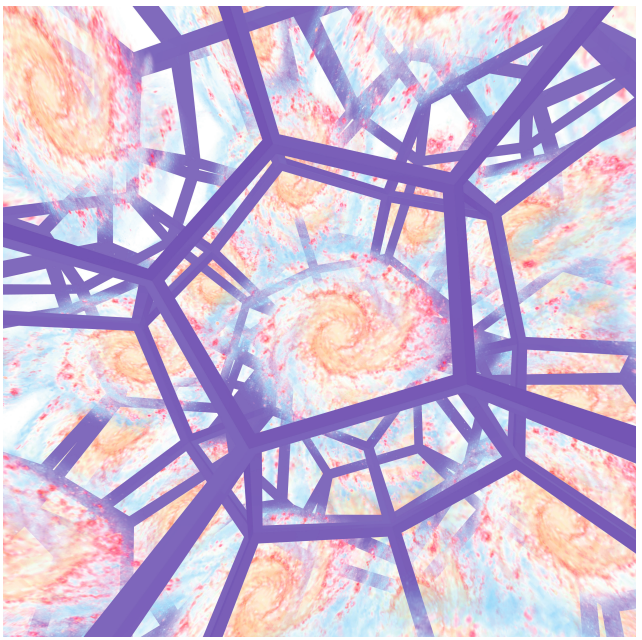
\includegraphics[scale=.40]{visdoc.png}
\caption{visão dentro dum universo de uma só galáxia modelado pelo dodecaedro de Poincaré}
\end{figure}
Poincaré concluiu o artigo em que apresentou seu contra-exemplo da seguinte maneira:

\blockquote{
Existem portanto dois laços na variedade que não são equivalentes a um ponto; portanto a variedade não pode ser homeomorfa a uma esfera. \par 
Em outras palavras... \emvioleta{[Ele enuncia novamente o resultado, explicando que o grupo fundamental não é trivial].} \par 
Permanece ainda uma questão a lidar: é possível que o grupo fundamental de uma variedade tri-dimensional poderia ser trivial, mas que a variedade não fosse homeomorfa à esfera tri-dimensional $\mathbb{S}^3$ \emvioleta{[Essa é a conjectura de Poincaré!]} \par 
Em outras palavras... \emvioleta{[Ele explica cuidadosamente, em termos do exemplo construído, o que precisaria acontecer para obter tal variedade].} \par 
Mas tal questão nos levaria longe demais.
 }
 A resposta negativa da conjectura só veio muito depois. Em dimensão $3$, ainda temos as três geometrias-modelo de curvatura constante - a saber, $\mathbb{S}^3$, $\mathbb{R}^3$ e $\mathbb{H}^3$. Mas não há esperança de uma classificação tão boa quanto em dimensão $2$: de fato, existem infinitas variedades tri-dimensionais que não admitem nenhuma métrica de curvatura seccional constante (considere, por exemplo, $\mathbb{S}^2 \times \mathbb{S}^1$, cujo recobrimento universal é $\mathbb{R}$). Cinco outras geometrias-modelos surgem de produtos cartesianos ou \quotes{torcidos} de geometrias de dimensão mais baixa:
\begin{itemize}
\item o produto $\mathbb{S}^2 \times \mathbb{R}$
\item o produto $\mathbb{H}^2 \times \mathbb{R}$
\item o recobrimento universal $\widetilde{S L}(2, \mathbb{R})$ (um fibrado torcido sobre $\mathbb{H}^2$)
\item o grupo de Heisenberg (um fibrado torcido sobre $\mathbb{R}^2$); e
\item a variedade Sol (um $\mathbb{T}^2$-fibrado torcido sobre $\mathbb{S}^1$)
\end{itemize}
A conjectura da geometrização de Thurston afirma que toda $3$-variedade fechada pode ser apropriadamente decomposta de maneira que cada pedaço da decomposição admita uma das geometrias citadas anteriormente. Mais precisamente, 
\begin{conjec} \textit{
Seja $\mm^3$ uma variedade fechada, orientável e prima (id est, não pode ser expressa como uma soma conexa não trivial - ou seja, com nenhum dos fatores sendo uma esfera - de duas variedades tri-dimensionais). Então existe um mergulho de uma união disjuntas de toros e garrafas de Klein  $\displaystyle{\cup_{i} T_i^2 \subset \mm}$ tal que cada componente do complemento admite uma métrica Riemanniana localmente homogênea e de volume finito.}
\end{conjec}
Diremos que uma superfície fechada $S \subset \mm^3$ de gênero $g \geq 1$ é incompressível se existe uma injeção de seu grupo fundamental $\pi_1(S)$ no grupo fundamental $\pi_1(\mm^3)$ de $\mm^3$. Pode-se provar que toros e garrafas de Klein são incompressíveis. Uma reformalização da conjectura é então que existe uma decomposição de $\mm^3$ ao longo de toros e garrafas de Klein incompressíveis em pedaços cujos interiores admitem métricas localmente homogêneas de volume finito. Uma vez que $3$-variedades fechadas de grupo fundamental finito não têm toros ou garrafas de Klein incompressíveis, em tais casos, tal decomposição é trivial. E como a única geometria modelo compacta é $\mathbb{S}^3$, concluímos que se $\pi_1(\mm^3)$ é finito então o recobrimento universal de $\mm^3$ é a esfera $\mathbb{S}^3$. \emph{A fortiori,}
\[
\text{geometrização de Thurston $\implies$ conjectura de Poincaré}
\]
Thurston verificou que uma grande classe de variedades, chamadas \emph{variedades de Haken}, satisfazia sua conjectura. Tal trabalho foi importantíssimo. Nas palavras de John Morgan, 
\blockquote{
Na minha perspectiva, antes do trabalho de Thurston em $3$-variedades hiperbólicas e sua formalização da Conjectura da Geometrização, não havia consenso entre os especialistas quanto à validade da conjectura de Poincaré. Depois do trabalho de Thurston (não obstante o fato de que o mesmo não tinha nenhuma consequência direta à Conjectura de Poincaré), se desenvolveu um consenso de que ambas a Conjectura de Poincaré e a Conjectura da Geometrização eram verdadeiras.
}
De maneira um pouco grosseira, o problema de classicação/geometrização para variedades fechadas pode ser resumido do seguinte modo: 
\begin{itemize}
\item  Dimensão $1$: qualquer variedade (conexa) de dimensão $1$ sem bordo é difeomorfa ou ao círculo $\mathbb{S}^1$ ou à reta real $\mathbb{R}$. A presença de bordo introduz os casos adicionais $[0, 1]$ e $[0, 1)$. Compacidade e a presença de bordo são portanto invariantes topológicos que juntos determinam completamente a topologia de variedades de dimensão $1$. Além disso, o problema de geometrização em dimensão $1$ é trivial: não existe um invariante geométrico intrínseco que distingua duas variedades quaisquer de dimensão $1$. 
\item Dimensão $2$: Toda superfície fechada de gênero $g$ admite uma métrica de curvatura Gaussiana constante $K$. Além disso, vale que $K > 0$ se e só se $g = 0$, que $K = 0$ se e só se $g = 1$, e que $K < 0$ se e só se $g \geq 2$. 
\item Dimensão $3$: resolvida por Perelman pela sua resolução positiva à conjectura da geometrização de Thurston.
\item Dimensão $4$: não é possível obter nada tão abrangente como em dimensões mais baixas. De fato, como todo grupo finitamente representado é o grupo fundamental de alguma variedade quadri-dimensional (para uma prova desse fato, veja \mycitep{GrupoQuadri}), classificar variedades fechadas quadri-dimensionais é de certa forma tão difícil quanto classificar tais grupos. Tal problema é conhecido como o problema da palavra para grupos, e foi demonstrado como indecidível. 
\end{itemize}
Uma variedade tri-dimensional fechada não pode ser imersa num espaço Euclidiano (na verdade, é simples provar que não existe imersão de qualquer variedade fechada em outra variedade não-compacta de mesma dimensão), e portanto visualizações fiéis das mesmas são impossíveis. Ainda assim, os esforços nesse sentido apresentados no fantástico livro \mycitep{JeffShapeOfSpace}, alguns dos quais apresentamos em seguida, são bastante satisfatórios. 
\begin{figure}[H]
\centering
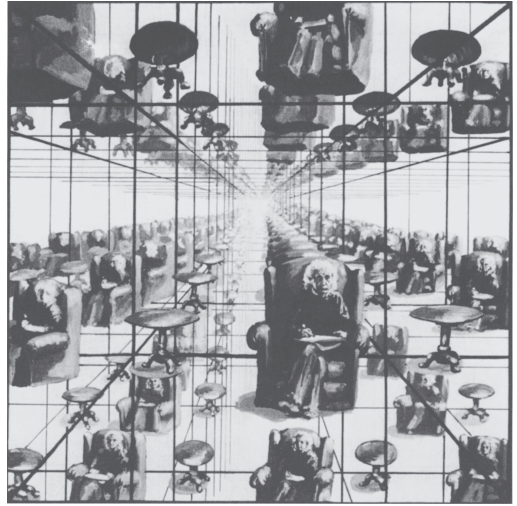
\includegraphics[scale=.6]{einsteintoro.png}
\caption{desenho artístico da visão num universo modelado pelo toro $\mathbb{T}^3$}
\end{figure}

\begin{figure}[H]
\centering
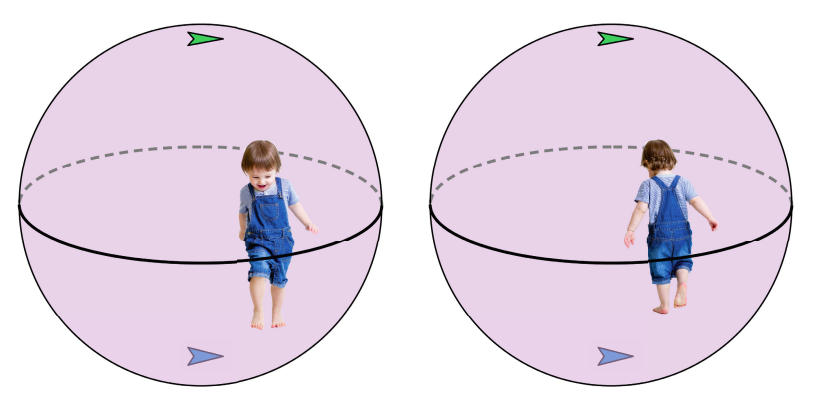
\includegraphics[scale=.5 ]{duasesf.png}
\caption{visualização de $\mathbb{S}^3$ como duas bolas colados ao longo do bordo $\mathbb{S}^2$}
\end{figure}

\begin{figure}[H]
\centering
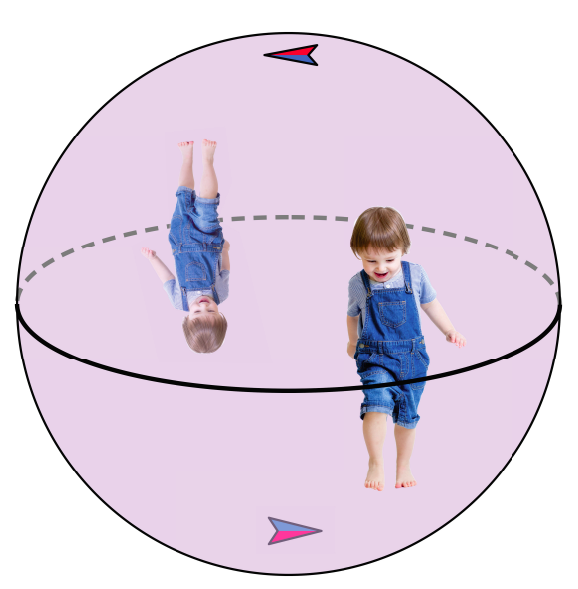
\includegraphics[scale=.3]{P3.png}
\caption{visualização de $\mathbb{R}\mathbb{P}^3$ como a esfera $\mathbb{S}^2$ com pontos antípodas identificados}
\end{figure}

\begin{figure}[H]
\centering
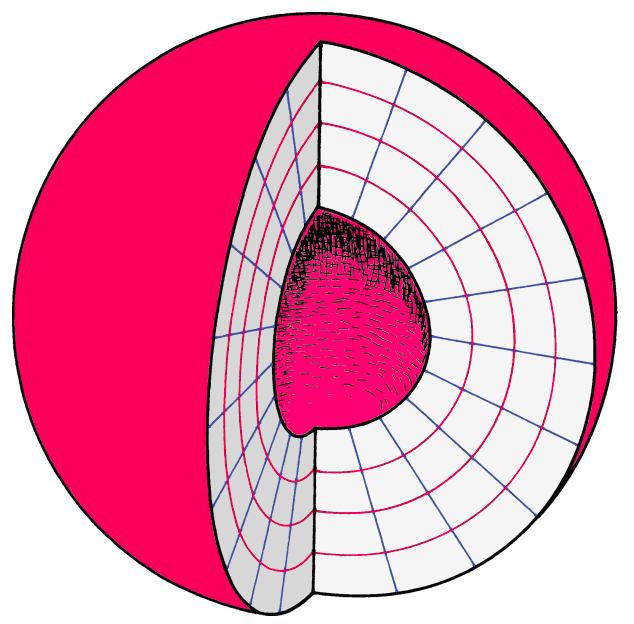
\includegraphics[scale=.4]{S2.png}
\caption{visualização de $\mathbb{S}^2 \times [0, 1]$ como uma bola com um centro oco. Para imaginar $\mathbb{S}^2 \times \mathbb{S}^1$, colamos o bordo esférico interno com o bordo esférico externo, fingindo (em constraste com um ser quadri-dimensional, que não teria que fingir) as várias camadas esféricas da casca vista acima têm todas o mesmo tamanho.}
\end{figure}

A princípio, um palpite ingênuo de como reconhecer a topologia do Universo sugeriria usar telescópios para procurar por cópias de nossa galáxia no céu. Se víssemos táis cópias, poderíamos determinar as \quotes{colas} do domínio fundamental do Universo e portanto sua topologia (as cópias vistas em um Universo modelado pelo toro $\mathbb{T}^3$ seriam diferentes das vistas em um universo modelado pelo dodecaedro de Poincaré, por exemplo). E se, por exemplo, uma das várias galáxias muito distantes descobertas até agora fosse na verdade a própria Via Láctea? Infelizmente, tal técnica não é nada promissora: detectar cópias do mesmo objeto (quasares, explosões de raios gama, outras galáxias, etc...) é inviável devido à finitude da velocidade da luz, que faz com que, na prática, \quotes{viajemos} ao passado ao olhar em telescópios. Como galáxias evoluem dramaticamente com o passar do tempo e o Universo observável é absurdamente enorme, é extremamente improvável que esse método eventualmente tenha sucesso. \par 
Ainda assim, a busca da resposta da \cref{FibUniverso} constitui um assunto de pesquisa muito ativo na Física, e outros métodos mais promissores, que usam fortemente Geometria Riemanniana, têm sido desenvolvidos recentemente. Veja, por exemplo, \mycitep{CosmicTopology} - a Mãe Natureza, em toda sua bondade e generosidade, nos forneceu a base de alguns de tais métodos via a radiação cósmica de fundo em micro-ondas, que sugere que o Universo pode ser modelado por uma forma espacial (justificando muito bem tal nome). Segundo experimentos recentes, há evidências consistentes com um Universo modelo por uma variedade tri-dimensional plana (\emph{id est}, curvatura seccional identicamente nula), das quais em dimensão $3$ só existem dezoito (dez orientáveis e oito não orientáveis, conforme provado em \mycitep{JosephWolf}). Devido à equação \cref{efe}, tais modelos são boas aproximações globais mas não são completamente fiéis (o que, novamente, não constitui uma grande perda de generalidade - a própria Terra também não é uma esfera, mas pode ser fielmente modelada por $\mathbb{S}^2$). 



\begin{thebibliography}{9}

{\bfseries
\color{teal}


\bibitem{ivoQ}
\bl{
\href{https://math.stackexchange.com/questions/4487531/why-isnt-the-dimension-of-the-space-of-curvature-like-tensors-equal-to-the-dime}{Why isn't the dimension of the space of curvature-like tensors equal to the dimension of the Grassmannian?}
}
\bibitem{foster}
\bl{\textbf{Foster, J.; Nightingale, J.D.;} \emph{A Short Course in General Relativity,} Springer, 2006.}


\bibitem{McMillan}
\bl{\textbf{McMillan, D. R., Jr.} Some contractible open $3$-manifolds. \emph{Trans. Amer. Math. Soc.} 102 (1962), 373--382. \href{https://mathscinet.ams.org/mathscinet-getitem?mr=137105}{\textbf{MR0137105}}}

\bibitem{Donal}
\bl{\textbf{Donal O'Shea}, \emph{The Poincaré Conjecture: In Search of the Shape of the Universe}}

\bibitem{Arnold}
\bl{\textbf{Arnold, Vladimir I.} On Teaching Mathematics. (Polonês) Traduzido do russo por Danuta Śledziewska-Blocka. \emph{Wiadom. Mat.} 37 (2001), 17--26.}

\bibitem{PEN1}
\bl{\textbf{Roger Penrose,} \emph{The Emperor's New Mind,} Oxford University Press, $1990$; Oxford Landmark Series, $2016$, pp.204-205.}

\bibitem{PEN2}
\bl{\textbf{Roger Penrose}, \textit{The Road to Reality: A Complete Guide to the Laws of the Universe}}

\bibitem{RIEMANN}
\bl{\textbf{Riemann}, \emph{On the Hypothesis Which Lie At the Bases of Geometry*. Nature} \textbf{8,} 36-37 (1873). \href{https://doi.org/10.1038/008036a0}{\textbf{https://doi.org/10.1038/008036a0}}}


\bibitem{POINCHYP}
\bl{\textbf{Poincaré}, \quotes{Science and Hypothesis}, \emph{The Value of Science: Essential Writings of Henri Poincaré, } ed. Stephen Jay Gould (New York: The Modern Library 2001), p.56.}



\bibitem{dodecaedro}
\bl{\textbf{C.Weber e H.Seifert}, \quotes{Die beiden Dodekaedraume,} \emph{Mathematische Zeitschrift} 37, no. 2 (1933).}

\bibitem{ArtDodecaedro}
\bl{\textbf{Luminet, J.-P., J.R. Weeks, A. Riazuelo, R. Lehoucq, R., and J.-P. Uzan.} \emph{Dodecahedral space topology as an explanation for weak wide-angle temperaure correlations in the cosmic microwave background.} Nature, (2003), \textbf{425}, 593-95.}

\bibitem{JeffShapeOfSpace}
\bl{\textbf{Jeffrey Weeks,} The shape of space.}

\bibitem{CosmicTopology}
\bl{\textbf{Michael P. Hitchman,} \href{https://mphitchman.com/}{\textbf{\textit{Geometry with an Introduction to Cosmic Topology.}}}}

\bibitem{JosephWolf}
\bl{\textbf{Joseph Wolf}, \emph{Spaces of Constant Curvature.}}

\bibitem{GrupoQuadri}
\bl{\textbf{John Stillwell}, \textit{Classical Topology and Combinatorial Group Theory,} GTM 72, Springer-Verlag.}





}




\end{thebibliography}

\end{document}
